\newpage
\appendix
\onecolumn 

\section{Evaluation Details and Additional Results} 

\subsection{Experimental Details} 
BubbleSpec is implemented on top of \texttt{Verl-0.5.0.dev0}, using \texttt{vLLM-v0.10.1} as the rollout backend. The tensor-parallel size is set to $1$. In general, smaller tensor-parallel sizes reduce inter-GPU communication overhead, but also decrease the available GPU memory for the KV cache, which can trigger runtime KV-cache swapping and request preemption. In such cases, long-tail requests may require more decoding steps. We therefore recommend choosing the smallest tensor-parallel size that does not incur severe KV-cache swapping.

For cross data-parallel rank synchronization, we use a Ray actor as a centralized coordinator. The unified attention implementation adopts TensorRT operators from FlashInfer, and the suffix-tree decoding is based on Arctic-Inference. We set the GPU memory utilization to $0.7$ and enable both the chunked prefill and CUDA graph modes of vLLM. The maximum number of batched tokens for rollout is set to $64\mathrm{k}$. Rollout sampling uses temperature $1.0$ and top\_p $1.0$.

For policy updates, we adopt the AdamW optimizer with a learning rate of $1\mathrm{e}{-6}$ and weight decay of $0.01$. For all samples, we use a rule-based reward manager. Specifically, we employ \texttt{math-verify} for answer extraction and verification against the ground truth. We do not include a KL-regularization term in either the loss or the reward. The PPO update mini-batch size is the same as the training batch size, \ie, training is conducted in an on-policy manner.

Qwen3-1.7B and Qwen3-4B are trained under the thinking mode. Qwen2.5-VL-7B-Instruct does not natively possess strong complex mathematical reasoning or long-chain-of-thought capabilities, so its RL training starts from a checkpoint obtained after SFT on the AceReason dataset. For both training and evaluation, all models use the following system prompt and the following chat template:

\begin{tcolorbox}[
    colback=Teal!10!white, 
    colframe=Teal,
    coltitle=Base,
    title = {System Prompt}
]
You FIRST think about the reasoning process as an internal monologue and then provide the final answer. The reasoning process MUST BE enclosed within \texttt{<think>} \texttt{</think>} tags. The final answer MUST BE put in \verb|\boxed{}|. 
\end{tcolorbox}

\begin{tcolorbox}[
    colback=Teal!10!white, 
    colframe=Teal,
    coltitle=Base,
    title = {Chat Template}
]
\{question\}\\
Please reason step by step, and put your final answer within \textbackslash boxed\{\}.
\end{tcolorbox}

\subsection{\yuhang{Speculative Decoding Pseudocode}}
\label{sec:spec_details}

For completeness, we provide the full BubbleSpec rollout procedure in Algorithm~\ref{alg:bubblespec_rollout}, including draft retrieval from the suffix tree, sequential verification under the current policy, acceptance/rejection handling, and fallback decoding after the first rejection. This pseudocode clarifies that BubbleSpec uses the retrieved continuation as a deterministic speculative proposal, while preserving the exact target rollout distribution through token-wise acceptance and residual resampling.

\begin{algorithm}[t]
\caption{BubbleSpec Rollout with Deterministic Draft Verification}
\label{alg:bubblespec_rollout}
\small
\begin{algorithmic}[1]
\REQUIRE Prompt $x_{1:m}$, target policy $\pi$, suffix tree $\mathcal{T}$, maximum generation length $L$
\ENSURE Rollout $y$

\STATE $y \leftarrow x_{1:m}$
\WHILE{$|y| < L$ and not EOS}
    \STATE Retrieve a draft block $\tilde{d} = (\tilde{x}_1,\dots,\tilde{x}_K)$ from $\mathcal{T}$ using prefix $y$
    \IF{$\tilde{d}$ is empty}
        \STATE Sample $x \sim \pi(\cdot \mid y)$
        \STATE $y \leftarrow y \circ x$
        \STATE \textbf{continue}
    \ENDIF

    \STATE $\textit{acceptedAll} \leftarrow \textbf{true}$
    \FOR{$t = 1$ to $K$}
        \STATE Let $p_t(\cdot)$ be the target decoding distribution under prefix $y$
        \STATE $a \leftarrow \tilde{x}_t$
        \STATE Accept $a$ with probability $p_t(a)$
        \IF{accepted}
            \STATE $y \leftarrow y \circ a$
            \IF{$a$ is EOS}
                \STATE \textbf{break}
            \ENDIF
        \ELSE
            \STATE Sample $x \sim r_t(\cdot)$, where
            \[
            r_t(x)=\frac{p_t(x)\mathbf{1}[x\neq a]}{1-p_t(a)}
            \]
            \STATE $y \leftarrow y \circ x$
            \STATE $\textit{acceptedAll} \leftarrow \textbf{false}$
            \STATE \textbf{break}
        \ENDIF
    \ENDFOR

    \IF{$\textit{acceptedAll}$ and last token is not EOS}
        \STATE \textbf{continue} \COMMENT{retrieve a new draft block from the extended prefix}
    \ENDIF
\ENDWHILE
\STATE \textbf{return} $y$
\end{algorithmic}
\end{algorithm}




\subsection{Analysis of Utilizing Intra-GPU Bubbles}
% Please add the following required packages to your document preamble:
% \usepackage{booktabs}
% \usepackage{multirow}
% \usepackage{graphicx}
\begin{table}[htbp]
\centering
\caption{Comparison of BubbleSpec using inter-gpu vs. intra-gpu bubbles.}
\label{tab:intra_bubble_comp}
\resizebox{0.9\textwidth}{!}{%
\begin{tabular}{@{}lccccc@{}}
\toprule
\multirow{2}{*}{\textbf{Method}} & \multirow{2}{*}{\textbf{Rollout Time (s)}} & \multicolumn{2}{c}{\textbf{Rollout Bubble Time (s)}} & \multicolumn{2}{c}{\textbf{Draft Response Length}} \\ \cmidrule(l){3-6} 
 &  & \textbf{Average} & \textbf{Maximum} & \textbf{Average} & \textbf{Maximum} \\ \midrule
BubbleSpec w/. Inter-GPU Bubble & 167.6 & 61.9 & 109.1 & 4169 & 24029 \\
BubbleSpec w/. Intra-GPU Bubble & 232.8 & 89.1 & 162.5 & 4524 & 26067 \\ \bottomrule
\end{tabular}%
}
\end{table}
We analyze the effect of utilizing intra-GPU bubbles in this section using Qwen3-1.7B. Specifically, when the active batch size is below the threshold of 8, we exploit intra-GPU bubbles on 6 out of 8 ranks, in the order in which their active batch size falls below 8. As shown in \autoref{tab:intra_bubble_comp}, compared with utilizing only inter-GPU bubbles, additionally utilizing intra-GPU bubbles allows us to make better use of otherwise idle GPU time. However, this does not translate into a direct increase in the draft response length. Therefore, we argue that exploiting inter-GPU bubbles alone is sufficient to provide good coverage for next-step response generation.

In addition, we observe that utilizing intra-GPU bubbles leads to significantly longer rollout time. This is due to interference with the current batch’s generation: adding next-batch prompts increases the effective batch size and slows down the decoding of the current batch. To illustrate this, we record the latest finish time among ranks that utilize inter-GPU bubbles and ranks that do not, respectively, as shown in \autoref{fig:intra_bubble_completion}. We find that ranks that are faster in earlier generation stages can actually complete later than initially slower ranks, due to both the unpredictable LLM output length and intra-GPU interference. We argue that, to efficiently utilize intra-GPU bubbles without slowing down the current batch, techniques such as intra-GPU sharing and isolation need to be employed~\cite{nova}. Since the LLM decoding stage is memory-bound, this isolation should target not only compute resources but, more importantly, the GPU main memory bandwidth.


\begin{figure*}[t!]
    \centering
    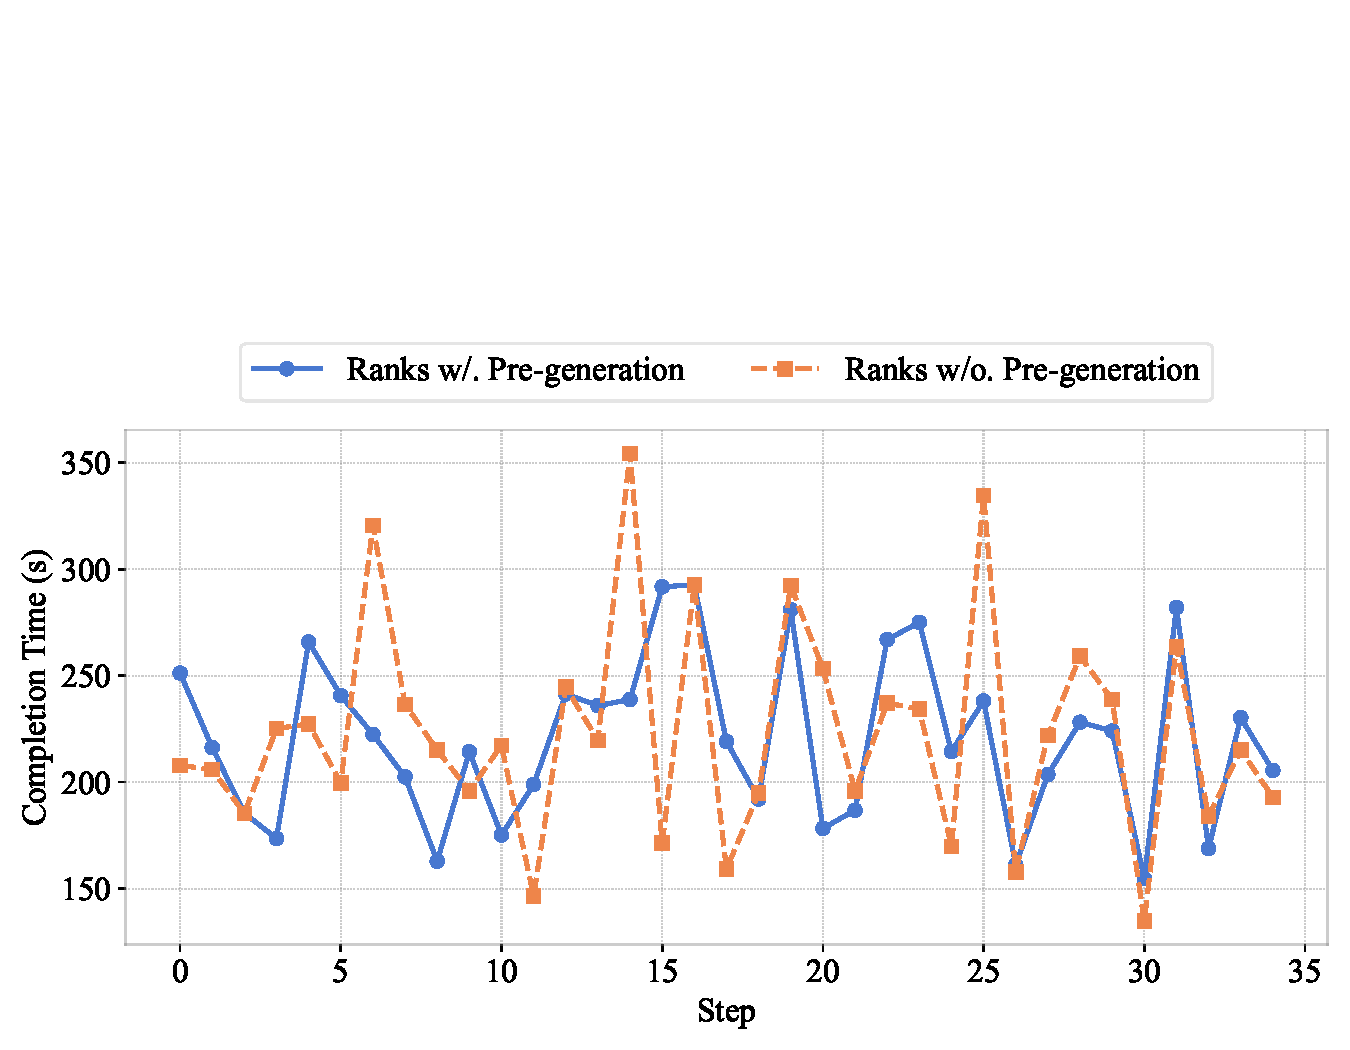
\includegraphics[width=0.85\linewidth]{appendix_arts/intra_bubble_vis.pdf}
    \caption{Latest completion time among ranks with and without response pre-generation.}
    \label{fig:intra_bubble_completion}
\end{figure*}

\subsection{Experiments on More RL Algorithms} 
% Please add the following required packages to your document preamble:
% \usepackage{booktabs}
% \usepackage{multirow}
% \usepackage{graphicx}
\begin{table}[t!]
\centering
\caption{BubbleSpec performance on Qwen3-1.7B across different RL algorithms.}
\label{tab:algo_comp}
\resizebox{0.95\textwidth}{!}{%
\begin{tabular}{@{}lcccccccc@{}}
\toprule
\multirow{2}{*}{\textbf{Method}} & \multirow{2}{*}{\textbf{Rollout Time (s)}} & \multicolumn{2}{c}{\textbf{Decoding Steps}} & \multicolumn{2}{c}{\textbf{Response Length}} & \multicolumn{3}{c}{\textbf{Speculative Metrics}} \\ \cmidrule(l){3-9} 
 &  & \textbf{Average} & \textbf{Maximum} & \textbf{Average} & \textbf{Maximum} & \textbf{Accept. Length} & \textbf{Draft Length} & \textbf{Accept. Rate} \\ \midrule
SAPO & 167.6 & 2913 & 15908 & 6592 & 39685 & 2.15 & 3.84 & 29.4\% \\
GRPO & 176.3 & 3032 & 17297 & 6844 & 39189 & 2.13 & 3.83 & 29.5\% \\
GSPO & 174.4 & 3001 & 17742 & 6773 & 39580 & 2.14 & 3.83 & 29.8\% \\ \bottomrule
\end{tabular}%
}
\end{table}

We further evaluate BubbleSpec under additional RL algorithms in \autoref{tab:algo_comp}, including GRPO and GSPO, and observe broadly similar performance across algorithms. As a rollout optimization framework, BubbleSpec can be seamlessly integrated into a wide range of RL algorithms.




\subsection{Bubble Time in RL Training}
We report the average and maximum bubble times across DP ranks throughout training for the three models in \autoref{fig:bubble_time_appendix}. Both metrics remain substantial relative to the total rollout latency, providing ample time for draft pre-generation and ensuring sufficient diversity and length coverage of speculative drafts.

\begin{figure*}[t!]
    \centering
    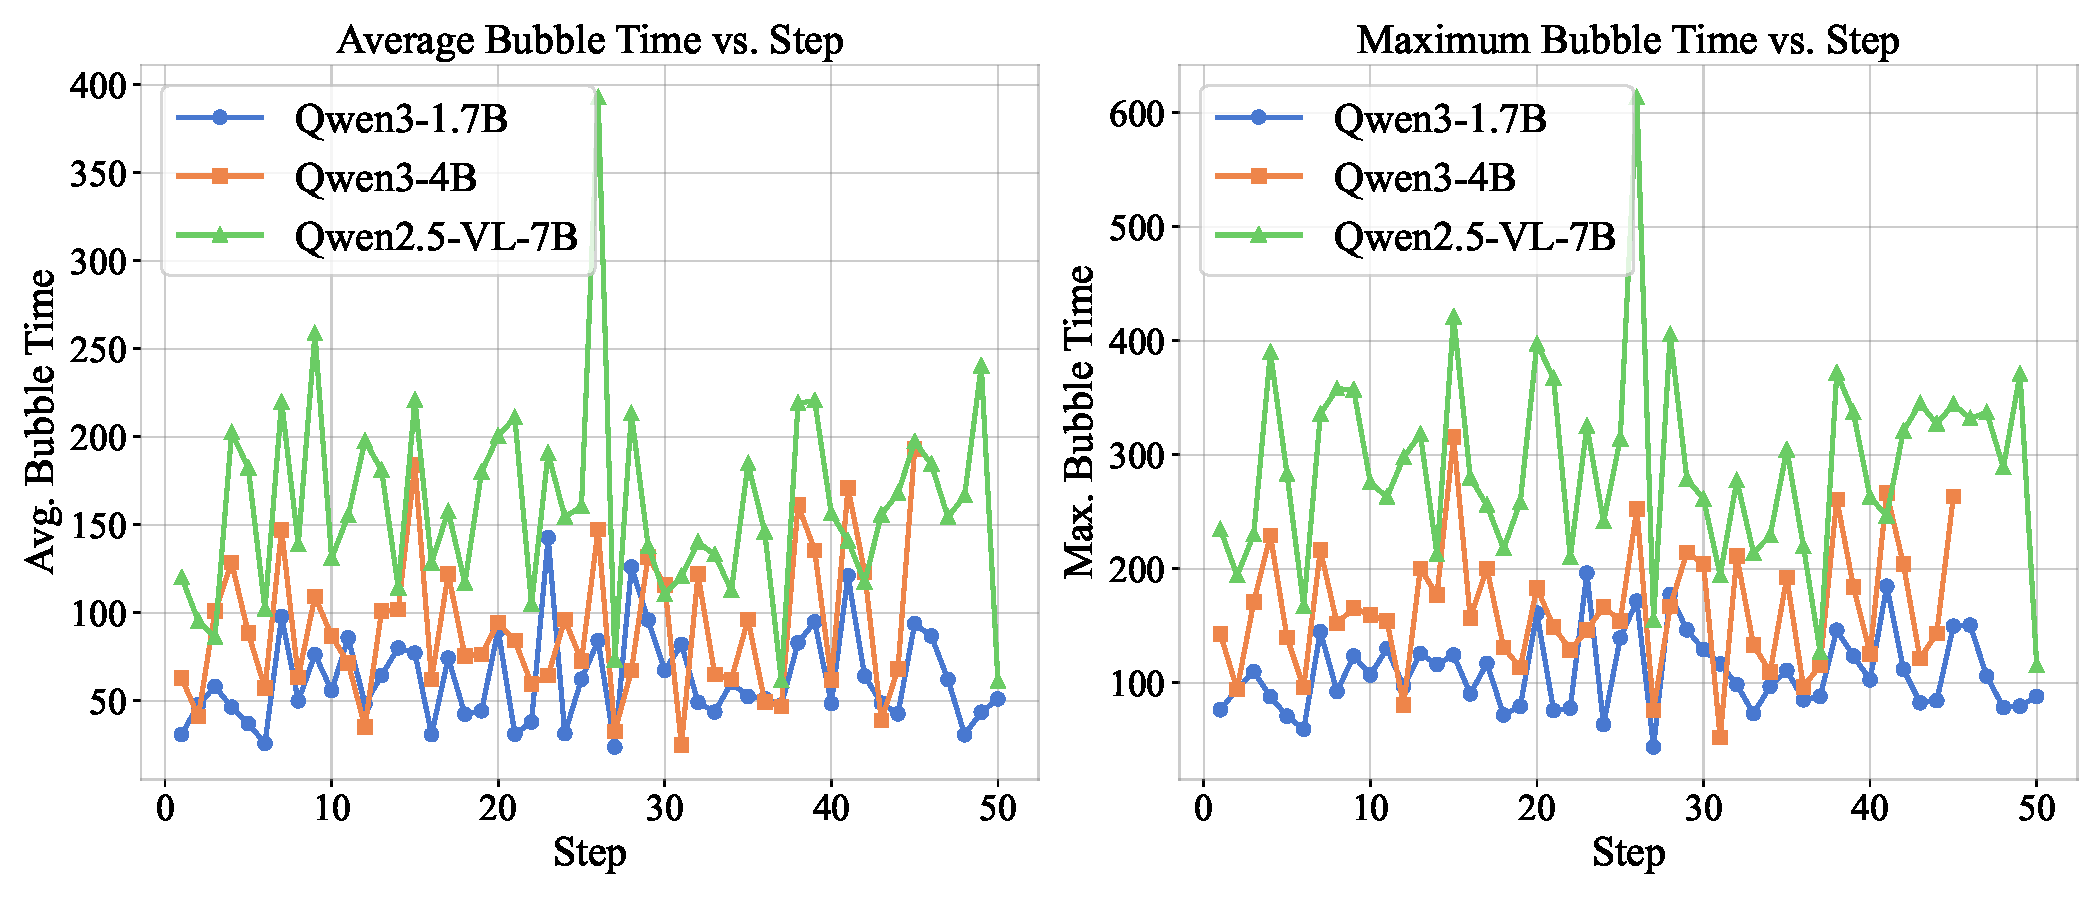
\includegraphics[width=0.95\linewidth]{appendix_arts/bubble_time_step.pdf}
    \caption{Average and maximum bubble time during training steps.}
    \label{fig:bubble_time_appendix}
\end{figure*}




\subsection{Test Accuracy on Qwen3-1.7B}
The AIME25 test accuracy of Qwen3-1.7B after 300 SAPO training steps is reported in \autoref{tab:acc_qwen3}, and closely matches that obtained with vanilla Verl training without speculative rollout acceleration.

% Please add the following required packages to your document preamble:
% \usepackage{booktabs}
% \usepackage{graphicx}
\begin{table}[htbp]
\centering
\caption{Test accuracy on AIME25 of Qwen3-1.7B after SAPO training for 300 steps.}
\label{tab:acc_qwen3}
\resizebox{0.9\textwidth}{!}{%
\begin{tabular}{@{}lccc@{}}
\toprule
Model & \textbf{Qwen3-1.7B} & \textbf{Qwen3-1.7B  (+BubbleSpec 300 steps)} & \textbf{Qwen3-1.7B  (+Verl 300 steps)} \\ \midrule
Score & 36.8 & 43.3 & 41.6 \\ \bottomrule
\end{tabular}%
}
\end{table}

